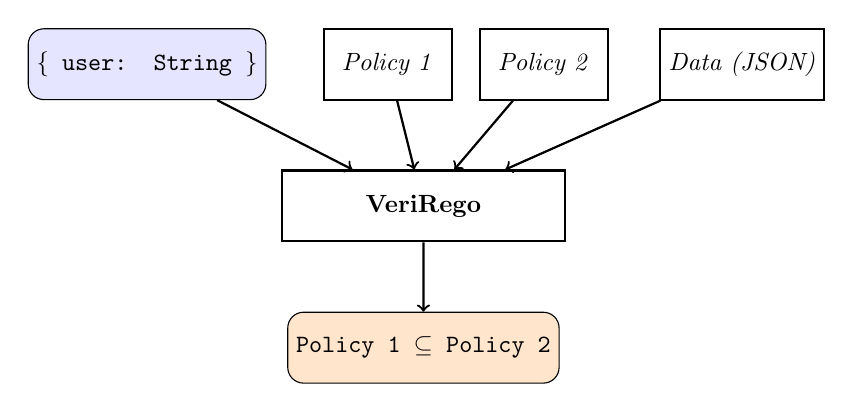
\begin{tikzpicture}[
            s/.style={draw,thick,rectangle,minimum height=10mm, minimum width=18mm},
            code/.style={draw,fill=blue!10,rectangle,minimum height=10mm, minimum width=18mm,rounded corners=2mm},
            e/.style={fill=gray!50},
            xsh/.style={xshift=15mm},
            transform shape, scale=0.9
        ]

        \tikzset{
            node distance=20mm,
        }

        \node[code] (input) {\texttt{\{ user: \textbf{String} \}}};
        \node[s,right of=input,xshift=14mm] (policy1) {\textit{Policy 1}};
        \node[s,right of=policy1,xshift=2mm] (policy) {\textit{Policy 2}};
        \node[s,right of=policy,xshift=8mm] (data) {\textit{Data (JSON)}};
        \node[s,below of=policy1,minimum width=40mm,xshift=5mm] (OPA) {\textbf{VeriRego}};
        \node[code,fill=orange!20,below of=OPA] (output) {\texttt{Policy 1 $\subseteq$ Policy 2}};

        \draw[->,thick]
            (input) edge (OPA)
            (policy1) edge (OPA)
            (policy) edge (OPA)
            (data) edge (OPA)
            (OPA) edge (output)
        ;

\end{tikzpicture}
